\documentclass{beamer}
%\documentclass[handout]{beamer}
\usefonttheme[onlymath]{serif}
% This file is a solution template for:
\usepackage{algorithm}
\usepackage{algpseudocode}
\usepackage{multicol}
% - Giving a talk on some subject.
% - The talk is between 15min and 45min long.
% - Style is ornate.



% Copyright 2004 by Till Tantau <tantau@users.sourceforge.net>.
%
% In principle, this file can be redistributed and/or modified under
% the terms of the GNU Public License, version 2.
%
% However, this file is supposed to be a template to be modified
% for your own needs. For this reason, if you use this file as a
% template and not specifically distribute it as part of a another
% package/program, I grant the extra permission to freely copy and
% modify this file as you see fit and even to delete this copyright
% notice. 

\mode<presentation>
{
  \usetheme{Warsaw}
  % or ...

  \setbeamercovered{transparent}
  % or whatever (possibly just delete it)
}
\setbeamertemplate{navigation symbols}{} 

\usepackage[english]{babel}
% or whatever

\usepackage[latin1]{inputenc}
% or whatever
\useoutertheme{default}

\usepackage{times}
\usepackage[T1]{fontenc}
% Or whatever. Note that the encoding and the font should match. If T1
% does not look nice, try deleting the line with the fontenc.
\newcommand{\beforeverb}{\footnotesize}
\newcommand{\afterverb}{\normalsize}

\title[Curve Fitting and Root Finding] % (optional, use only with long paper titles)
{Lecture 4}

\subtitle
{Curve Fitting} % (optional)

\author[Ying-Jer Kao] % (optional, use only with lots of authors)
{Ying-Jer Kao}
% - Use the \inst{?} command only if the authors have different
%   affiliation.

\institute[National Taiwan University] % (optional, but mostly needed)
{
  Department of Physics\\
 National Taiwan University
  }
% - Use the \inst command only if there are several affiliations.
% - Keep it simple, no one is interested in your street address.

\date[Numerical Analysis and Programming] % (optional)
{\today}

\subject{Talks}
% This is only inserted into the PDF information catalog. Can be left
% out. 



% If you have a file called "university-logo-filename.xxx", where xxx
% is a graphic format that can be processed by latex or pdflatex,
% resp., then you can add a logo as follows:

% \pgfdeclareimage[height=0.5cm]{university-logo}{university-logo-filename}
% \logo{\pgfuseimage{university-logo}}



% Delete this, if you do not want the table of contents to pop up at
% the beginning of each subsection:
%\AtBeginSubsection[]
%{
%  \begin{frame}<beamer>{Outline}
%    \tableofcontents[currentsection,currentsubsection]
%  \end{frame}
%}


% If you wish to uncover everything in a step-wise fashion, uncomment
% the following command: 

%\beamerdefaultoverlayspecification{<+->}


\begin{document}

\begin{frame}
  \titlepage
\end{frame}

\begin{frame}{Outline}
  \tableofcontents
  % You might wish to add the option [pausesections]
\end{frame}


% Since this a solution template for a generic talk, very little can
% be said about how it should be structured. However, the talk length
% of between 15min and 45min and the theme suggest that you stick to
% the following rules:  

% - Exactly two or three sections (other than the summary).
% - At *most* three subsections per section.
% - Talk about 30s to 2min per frame. So there should be between about
%   15 and 30 frames, all told.
\section[Curve Fitting]{Curve Fitting}
\subsection{Introduction}
\begin{frame}{Introduction}
\begin{itemize}
\item Typical data obtained from experiments normally contain a significant amount of random noise due to measurement errors. 
\item It is desirable to find a smooth curve with a simple form that \alert{best} fits the data points. 
\end{itemize}
\begin{columns}
\begin{column}[b]{0.3\textwidth}
\begin{center}
\begin{tabular}{cc|cc}
\hline
$x_i$ & $y_i$ & $x_i$ & $y_i$
\\\hline
1 & 1.3 & 6 & 8.8\\
2 & 3.5 & 7 & 10.1 \\
3 & 4.2 & 8 & 12.5\\
4 & 5.0 & 9 & 13.0 \\
5 & 7.0 & 10 & 15.6\\
\hline
\end{tabular}
\end{center}
\end{column}
\begin{column}{0.6\textwidth}
\centerline{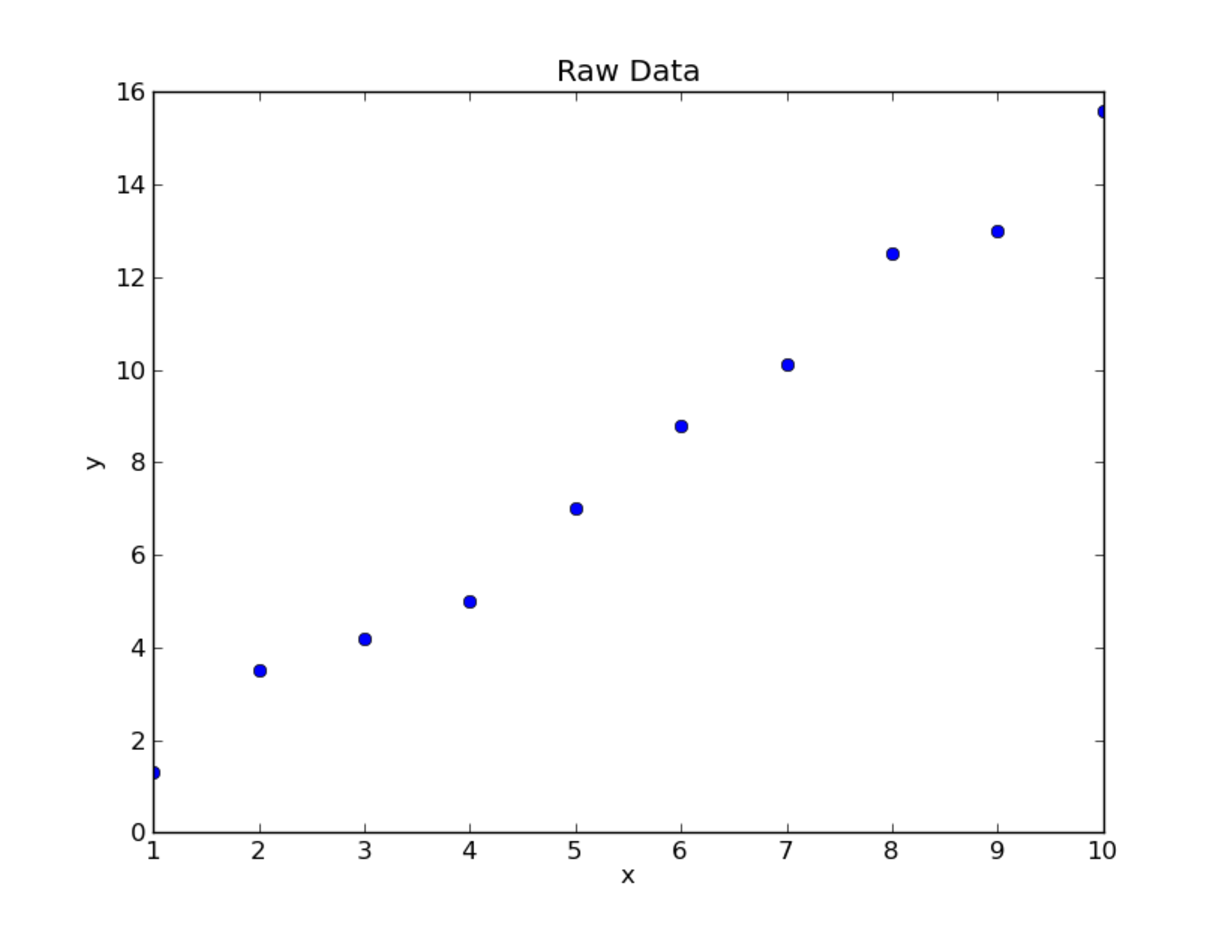
\includegraphics[width=\textwidth]{Lec11_fig1.pdf}}
\end{column}
\end{columns}
\end{frame}
\begin{frame}{Polynomial Interpolation}
\centerline{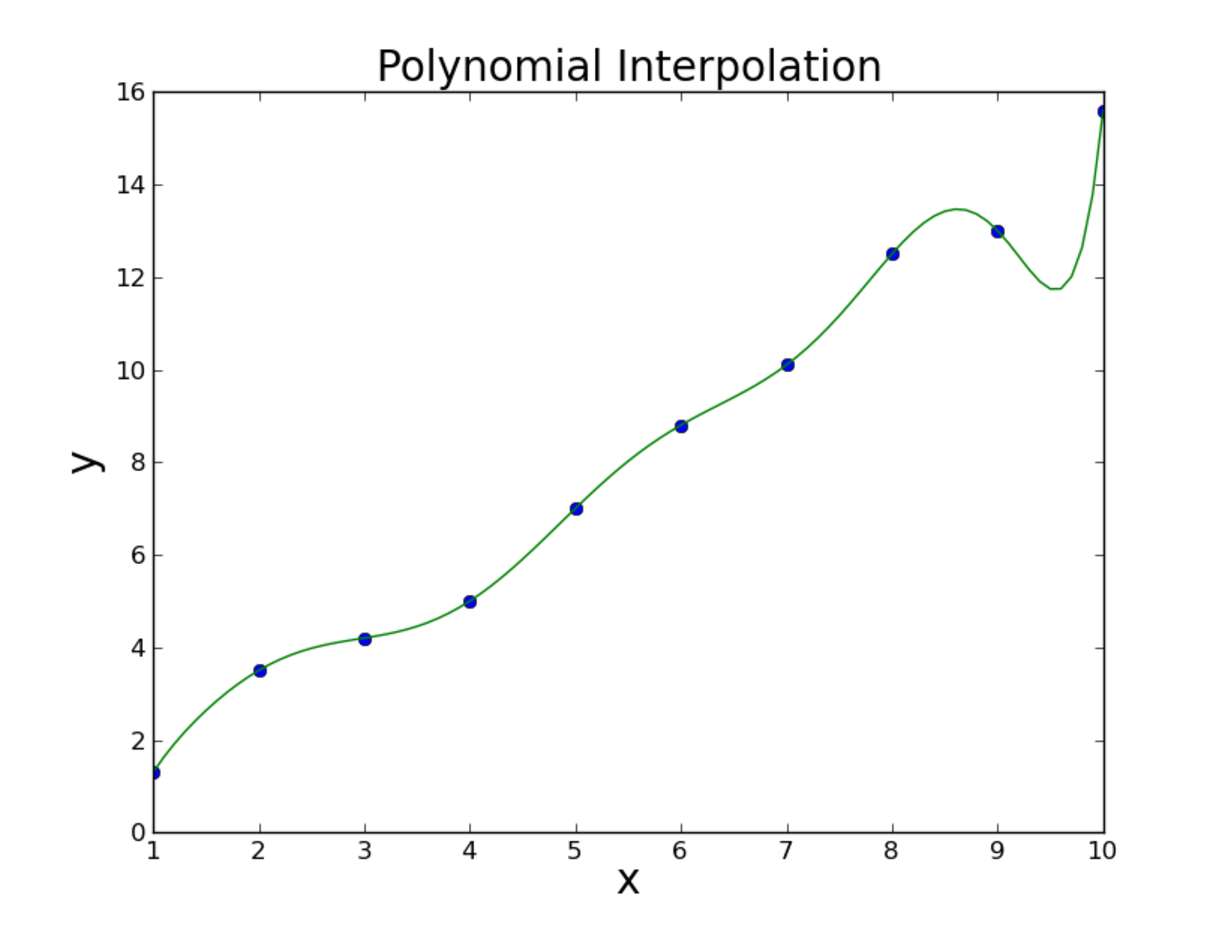
\includegraphics[width=0.6\textwidth]{Lec11_fig2.pdf}}

\begin{itemize}
\item The nine-degree polynomial is a \alert{poor} predictor of information between some data points. 
\item A better approach is to find the \alert{best approximating line}, even if it does not agree precisely with the data at \alert{any point}.
\end{itemize}
\end{frame}
\begin{frame}{Cubic Spline Interpolation}
\centerline{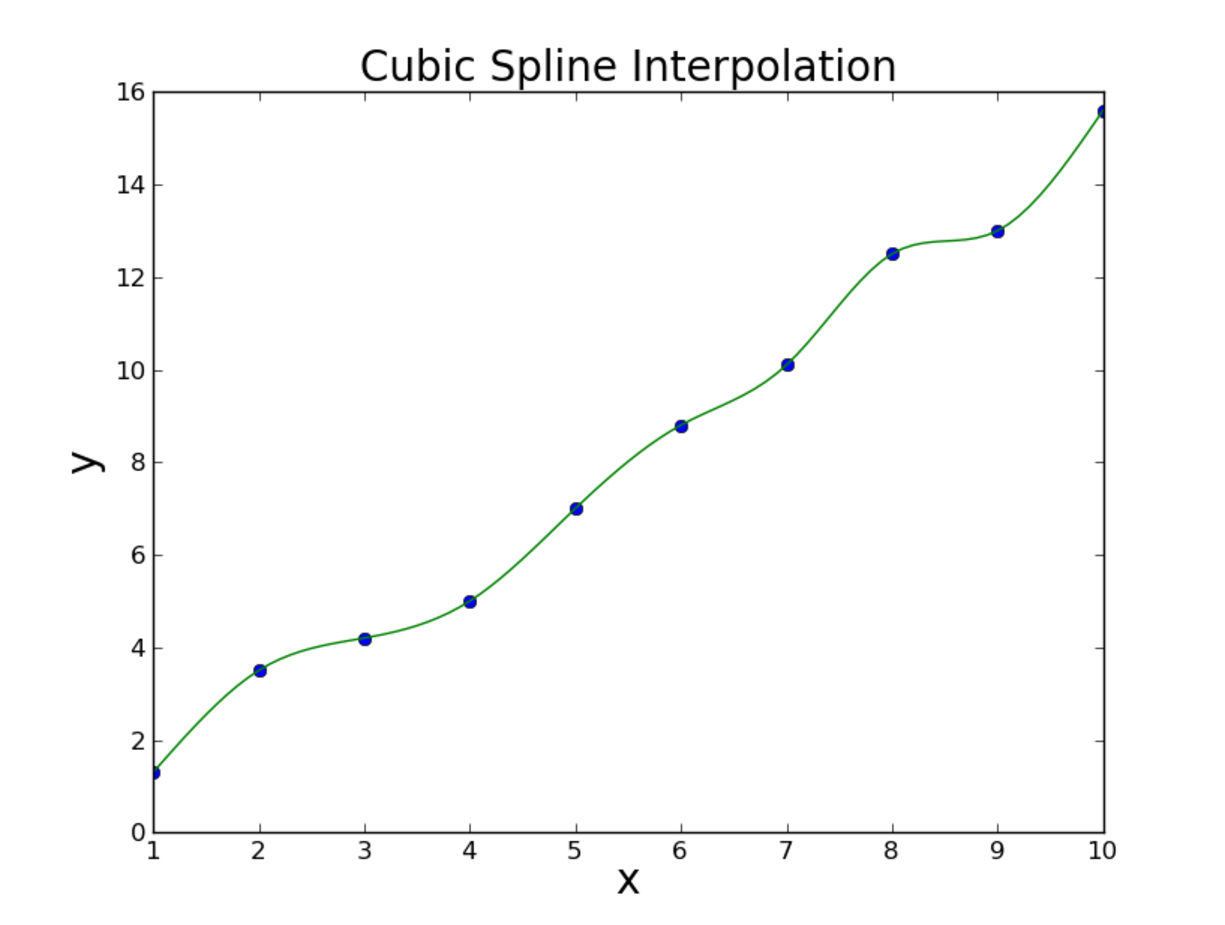
\includegraphics[width=0.65\textwidth]{Lec11_fig3.pdf}}

\begin{itemize}
\item Cubic-spline provides a better interpolation for the data.
\item However, it still does not capture the general trend of the data
\end{itemize}
\end{frame}
\subsection[Least-Squares Fit]{Least-Squares Fit}
\begin{frame}{Least-Squares Fit}
\begin{itemize}
\item  $f(x)=f(x;a_0,a_1,\ldots,a_m)$ is the function to be fitted to the $n+1$ data points $(x_i,y_i),i=0,1,\ldots,n$.
\item The form of $f(x)$ is predetermined, and the  $m+1$ parameters $a_0, a_1, \ldots, a_m$ are to be determined.
\item The best fit function is determined by the \alert{least-squares} fit, which minimizes
\[
S(a_0, a_1, a_2, \ldots, a_m) =\sum_{i=0}^n[y_i-f(x_i)]^2
\]
with respect to $a_j$. 
\end{itemize}
\end{frame}

\begin{frame}{Least-Squares Fit}
\begin{itemize}
\item The optimal values of the parameters are given by the solution of the $m$ equations
\[
\frac{\partial S}{\partial a_k}=0,\quad k=0,1,\ldots,m
\]
\item The \alert{residuals} $r_i=y_i-f(x_i)$ represent the discrepancy between the data points and the fitting function at $x_i$.
\item The fitting function $f(x)$ is often chosen as a linear combination of specific functions $f_j(x)$
\[
f(x)=a_0 f_0(x)+a_1 f_1(x) + \cdots+ a_m f_m(x)
\]
\item The \alert{standard deviation} estimates spread of the data about the fitting curve, defined as
\[
\sigma=\sqrt{\frac{S}{n-m}}
\] 
\end{itemize}
\end{frame}
\begin{frame}{Fitting Linear Forms}
\begin{itemize} 
\item Consider the linear form 
\[
f(x)=a_0 f_0(x)+a_1 f_1(x) + \cdots+ a_m f_m(x)= 
\sum_{j=0}^m a_j \,f_j(x)
\]
\item The least-squares error is given as
\[
S=\sum_{i=0}^n \left[y_i-\sum_{j=0}^m a_j \,f_j(x_i) \right]^2
\]
and 
\[
\frac{\partial S}{\partial a_k}=-2\left\{\sum_{i=0}^n \left[ y_i -\sum_{j=0}^m a_j \,f_j(x_i)\right] f_k(x_i)\right\}=0,\quad k=0,1,\ldots,m
\]
\end{itemize}
\end{frame}
\begin{frame}{Fitting Linear Forms}
\begin{itemize} 
\item $a_j$'s satisfy the \alert{normal equations} of the least-squares fit, 
\[
\sum_{j=0}^m \left[\sum_{i=0}^n f_j(x_i)\, f_k(x_i)\right] a_j =\sum_{i=0}^n f_k(x_i) y_i, \quad k=0,1,\ldots,m
\]
\item In matrix notation
\[
\mathbf{Aa}=\mathbf{b}
\]
where the matrix elements of $\mathbf{A}$ and $\mathbf{b}$ are
\[
A_{kj}=\sum_{i=0}^n f_j(x_i)\, f_k (x_i)\quad\quad b_k =\sum_{i=0}^n f_k(x_i) y_i
\]
\item The coefficient matrix is symmetric, $A_{kj}=A_{jk}$.
\end{itemize}
\end{frame}
\begin{frame}{Polynomial Fit}
\begin{itemize}
\item Consider the case where the fitting function $f(x)$ is a polynomial, 
\[
f(x)=a_0+a_1x+a_2x^2+\cdots+a_m x^m =\sum_{j=0}^m a_j \,x^j
\]
\item The basis functions are $f_j(x)=x^j, (j=0, 1, \ldots,m)$, and we obtain the form of the coefficient matrix $\mathbf{A}$ and the constant 
vector $\mathbf{b}$ 
\[
A_{kj}=\sum_{i=0}^n x_i ^{j+k}\quad b_k=\sum_{i=0}^n x_i^k y_i
\]
\end{itemize}
\end{frame}
\begin{frame}{Polynomial Fit}
\begin{itemize}
\item The normal equations to be solved for $a_i$ are 
\beforeverb
\[
\left[
\begin{array}{lllll}
n & \sum x_i & \sum x_i^2 & \cdots & \sum x_i^m \\
\sum x_i & \sum x_i^2 &  \sum x_i^3& \cdots  & \sum x_i^{m+1}\\
\vdots & \vdots & \vdots & \ddots &\vdots \\
\sum x_{m-1} & \sum x_i^m  & \sum x_i^{m+1} & \cdots & \sum x_i^{2m}
\end{array}
\right] \left[
\begin{array}{l}
a_0 \\
a_1 \\
\vdots\\
a_m
\end{array}
\right]
=\left[
\begin{array}{l}
\sum x_i \\
\sum x_i y_i \\
\vdots\\
\sum x_i^m y_i
\end{array}
\right]
\]
\afterverb
\item The normal equations become progressively ill conditioned with increasing $m$. 
\item Normally, only \alert{ low-order polynomials} are useful in curve fitting. 
\item Polynomials of high order are not recommended, because they tend to reproduce the noise inherent in the data.
\end{itemize}
\end{frame}
\begin{frame}{Weighted  Data}
\begin{itemize}
\item There are occasions when our confidence in the accuracy of data varies from point to point.
\item For example, in some region the instrument has higher sensitivity compared to other region, or more measurements are performed to reduce the statistical errors than other regions. 
\item We want to \alert{weight} the data and minimize the sum of \alert{weighted residuals}
\[
S(a_0,a_1, \ldots,a_m)=\sum_{i=0}^mW_i [y_i-f(x_i)]^2
\]
\item The fitting function $f(x)$ will be  closer to the data points that have higher weights.
\end{itemize}
\end{frame}
\begin{frame}{Weighted Linear-Squares Fit}
\begin{itemize}
\item Consider the linear form, the weighted normal equations are given by
\beforeverb
\[
\sum_{j=0}^m \left[\sum_{i=0}^n W_i f_j(x_i)\, f_k(x_i)\right] a_j =\sum_{i=0}^n W_i f_k(x_i) y_i, \quad k=0,1,\ldots,m
\]
\afterverb
\item For $f(x)=a+bx$, the normal equations are
\beforeverb
\begin{align*}
a \sum_{i=0}^n W_i+ b \sum_{i=0}^n W_i x_i &= \sum_{i=0}^n  W_i y_i \\
a \sum_{i=0}^n W_i x_i+b\sum_{i=0}^n W_i x_i^2 &= \sum_{i=0}^n W_i x_i y_i
\end{align*}
\afterverb
and we obtain
\beforeverb
\begin{align*}
a&=\hat{y} - b \hat{x},\quad b=\frac{\sum W_i y_i (x_i-\hat{x})}{	\sum W_i x_i (x_i-\hat{x})}\\
\hat{x}&=\frac{\sum W_i x_i}{\sum W_i },\quad \hat{y}=\frac{\sum W_i y_i}{\sum W_i }
\end{align*}
\afterverb
\end{itemize}
\end{frame}
\begin{frame}{Fitting Exponential Functions}
\begin{itemize}
\item  Consider  the fitting function $f(x)=ae^{bx}$. 
\item The least-squares fit would lead to equations that are \alert{nonlinear} in $a$ and $b$.
\item A better way is to fit a new  function $F(x)=\ln f(x)=\ln a + b x$ to the set of data points $( x_i, \ln y_i) $.
\item However, the least-squares fit to the logarithm of the data is \alert{not quite the same} as the least-squares fit to the original data. 

\end{itemize}
\end{frame}
\begin{frame}{Fitting Exponential Functions}
\begin{itemize}
\item The residuals of the original fit are,
\[
r_i =y_i-f(x_i)=y_i - a e^{bx_i}
\]
and those of the logarithmic  fit are,
\begin{align*}
R_i &=\ln y_i-F(x_i)=\ln y_i-(\ln a + b x_i )\\
 &=\ln y_i - \ln(r_i-y_i)=\ln \left(1-\frac{r_i}{y_i}\right).
\end{align*}
\item Minimizing $\tilde{S}=\sum R_i^2$, we obtain the least-squares fit to the logarithm of the data. Using the approximation, $R_i\approx r_i/y_i$,  we find that weights of \alert{$1/y_i^2$} is introduced in the process.
\item We can fix this by applying the weights $W_i=y_i^2$ when fitting $F(x)$ to $(x_i,\ln y_i)$.
\end{itemize}
\end{frame}

\section[Root Finding]{Root Finding}
\subsection{Introduction}
\begin{frame}{Introduction}
\begin{itemize}
\item The root of a function $f(x)$ is the value of $x$ for which $f(x)=0$.
\item   The root of a function is also called a \alert{zero} or a \alert{solution} of the function.
\item  All methods of finding roots are iterative procedures that require a starting point.
\item In general, an equation might have any number of \alert{real} roots, including none, one, or many.
\item For example,$\sin x - x =0$ has a root at $x=0$, and $\tan x-x=0$ has roots at $x=0,\pm \pi, \pm 2\pi, \ldots$.
\end{itemize}

\end{frame}

\subsection{Bisection Method}
\begin{frame}{Bisection Method}
  \begin{itemize}
    \item The bisection method is a simple and robust method for finding the root of a function $f(x)$.
    \item The method requires that the function $f(x)$ be continuous and that the root be bracketed by two points $a$ and $b$.
    \item The method is based on the intermediate value theorem, which states that if a continuous function $f(x)$ has opposite signs at the endpoints of an interval, then there is at least one root in the interval.
  \end{itemize}
\end{frame}

\begin{frame}[fragile]{Bisection Method}
  \begin{multicols}{2}
  \scriptsize
    \begin{algorithmic}
    \Procedure{Bisection}{$f, a, b, n\_max, \varepsilon$}
      \State \textbf{Input:} $f, a, b, n\_max, \varepsilon$
      \State \textbf{Output:} Root of $f$ in $[a, b]$
      \State $fa \gets f(a)$
      \State $fb \gets f(b)$
      \If {$\text{sign}(fa) = \text{sign}(fb)$}
        \State \textbf{output} $a, b, fa, fb$
        \State \textbf{output} "function has same signs at $a$ and $b$"
        \State \textbf{return}
      \EndIf
      \State $error \gets b - a$
      \For {$n = 0$ to $n\_max$}
        \State $error \gets error / 2$
        \State $c \gets a + error$
        \State $fc \gets f(c)$
        \State \textbf{output} $n, c, fc, error$
        \If {$|error| < \varepsilon$}
          \State \textbf{output} "convergence"
          \State \textbf{return}
        \EndIf
        \If {$\text{sign}(fa) \neq \text{sign}(fc)$}
          \State $b \gets c$
          \State $fb \gets fc$
        \Else
          \State $a \gets c$
          \State $fa \gets fc$
        \EndIf
      \EndFor
    \EndProcedure
    \end{algorithmic}
  \end{multicols}
\end{frame}
\begin{frame}{Convergence Analysis}
  \centerline{ 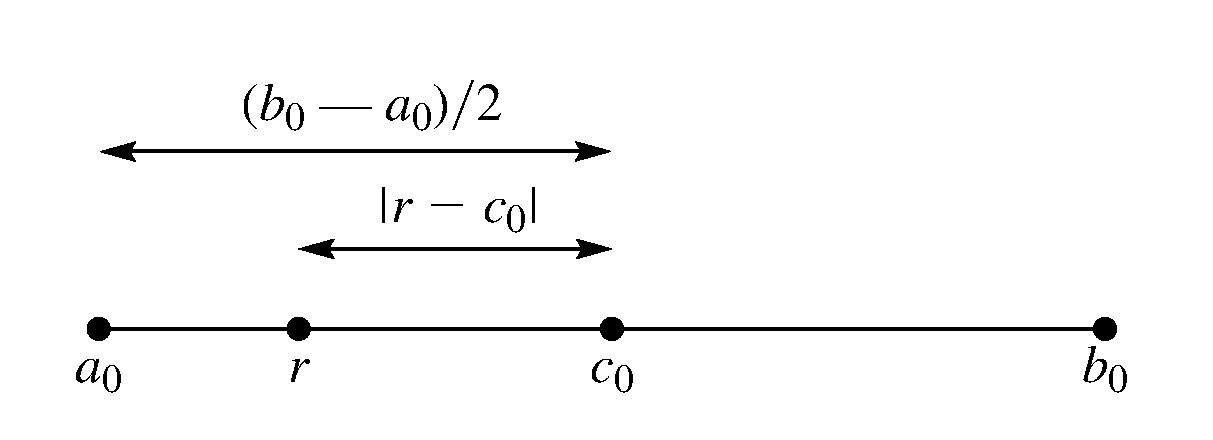
\includegraphics[height=1in]{Lec11_fig4.pdf}}
  \begin{itemize}
  \item If $f(a_0) f(b_0)<0$, then the root is bracketed by $a_0$ and $b_0$.
  \item If we use midpoint $c_0=(a_0+b_0)/2$ as our estimate for the solution $r$, then the error is $|r-c_0| \leq (b_0-a_0)/2$.
  \item  The error is reduced by a factor of 2 at each iteration, after $n$ iterations
  \[\left|r-c_n\right| \leqq \frac{b_0-a_0}{2^{n+1}} \]
  \end{itemize}
\end{frame}
\begin{frame}{Convergence Analysis}
\begin{block}{Theorem}
  If the bisection algorithm is applied to a continuous function $f$ on an interval $[a, b]$, 
  where $f(a) f(b)<0$, then, after $n$ steps, an approximate root will have been computed with 
  error at most $(b-a) / 2^{n+1}$.
  \end{block}
\begin{itemize}
\item If an error tolerance has been prescribed in advance, it is possible to determine the number of steps required in the bisection method.
\item If we want $\left|r-c_n\right|<\epsilon$, then we require that $(b_0-a_0)/2^{n+1}<\epsilon$, or $n>\log_2[(b_0-a_0)/\epsilon]-1$.
\end{itemize}
\end{frame}

\begin{frame}{When to use the Bisection Method}
\begin{itemize}
\item The bisection method is a robust method for finding the root of a function.
\item The method is guaranteed to converge to a root if the function is continuous and the root is bracketed by two points.
\item The method is slow compared to other methods, but it is reliable and easy to implement.
\item The bisection method is used to get close to the root before switching to a faster method.
\end{itemize}
\end{frame}
\subsection{Newton's Method}

\begin{frame}{Newton's Method}
\centerline{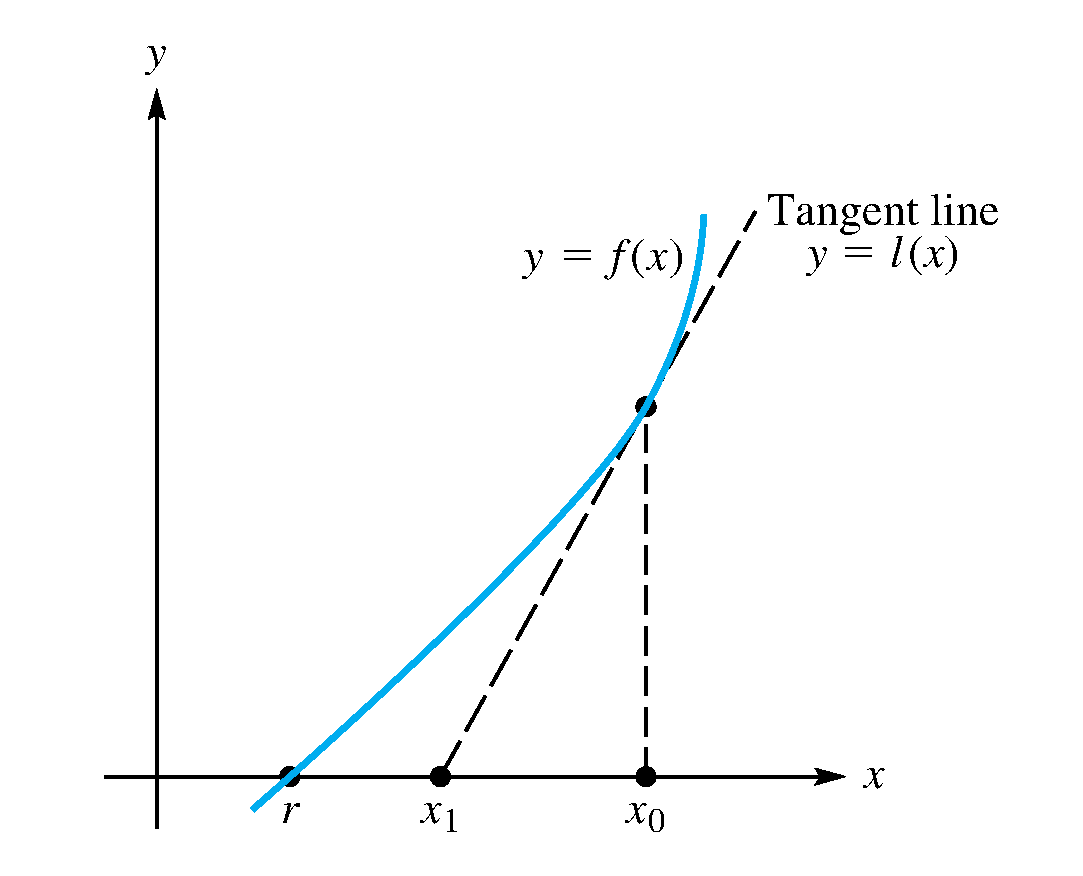
\includegraphics[height=1.2in]{Lec11_fig5.pdf}}  
\begin{itemize} 
  \item  Newton's method requires that the function $f(x)$ be differtiable.
  \item  At a point $(x_0, f (x_0))$, the tangent $l(x)$ is a  good approximation to the curve in the vicinity of that point,
 $$
l(x)=f^{\prime}\left(x_0\right)\left(x-x_0\right)+f\left(x_0\right),
$$
which intersects the $x$-axis at $x_1=x_0-\frac{f\left(x_0\right)}{f^{\prime}\left(x_0\right)}$.
\end{itemize}
\end{frame}
\begin{frame}{Newton's Method}
  \begin{itemize}
    \item If Newton's method is applied to the function $f(x)$, the iteration formula is
    $$
x_{n+1}=x_n-\frac{f\left(x_n\right)}{f^{\prime}\left(x_n\right)}, \quad \lim_{n \to \infty} x_n=r,
$$
    where $r$ is the root of $f(x)$. 
  \end{itemize}
\end{frame}

\begin{frame}[fragile]{Newton-Raphson Method}
  \scriptsize 
\begin{algorithmic}
\Procedure{Newton}{$f, f', x, n\_max, \varepsilon, \delta$}
  \State \textbf{Input:} $f, f', x, n\_max, \varepsilon, \delta$
  \State \textbf{Output:} Root of $f$
  \State $fx \gets f(x)$
  \State \textbf{output} $0, x, fx$
  \For {$n = 1$ to $n\_max$}
    \State $fp \gets f'(x)$
    \If {$|fp| < \delta$}
      \State \textbf{output} "small derivative"
      \State \textbf{return}
    \EndIf
    \State $d \gets fx / fp$
    \State $x \gets x - d$
    \State $fx \gets f(x)$
    \State \textbf{output} $n, x, fx$
    \If {$|d| < \varepsilon$}
      \State \textbf{output} "convergence"
      \State \textbf{return}
    \EndIf
  \EndFor
\EndProcedure
\end{algorithmic}
\end{frame}
\begin{frame}{Convergence Analysis}
  \begin{itemize}
    \item The error in the estimate $x_n$ is $|r-x_n| \leq |r-x_{n-1}|^2/|f^{\prime}(x_{n-1})|$, which converges quadratically.
    \item The error is reduced by a factor of $|f^{\prime}(x_{n-1})|$ at each iteration.
    \item If the error tolerance is $\epsilon$, then we require that $|r-x_n|<\epsilon$, or $|r-x_{n-1}|^2/|f^{\prime}(x_{n-1})|<\epsilon$.
    \item The number of iterations required to achieve the error tolerance is $n>\log_2(|r-x_0|/\epsilon)$.
  \end{itemize}
\end{frame}
\begin{frame}{Convergence Analysis}
  \begin{block}{Newton's Method Theorem}
    If $f, f^{\prime}$, and $f^{\prime \prime}$ are continuous in a neighborhood of a root $r$ of $f$ and if $f^{\prime}(r) \neq 0$, then there is a positive $\delta$ with the following property: If the initial point in Newton's method satisfies $\left|r-x_0\right| \leqq \delta$, then all subsequent points $x_n$ satisfy the same inequality, converge to $r$, and do so quadratically; that is,

$$
\left|r-x_{n+1}\right| \leqq c(\delta)\left|r-x_n\right|^2
$$
where $c(\delta)$ is a constant that depends on $\delta$.
  \end{block}
\end{frame}
\begin{frame}{Choice of Initial Guess}
  \centerline{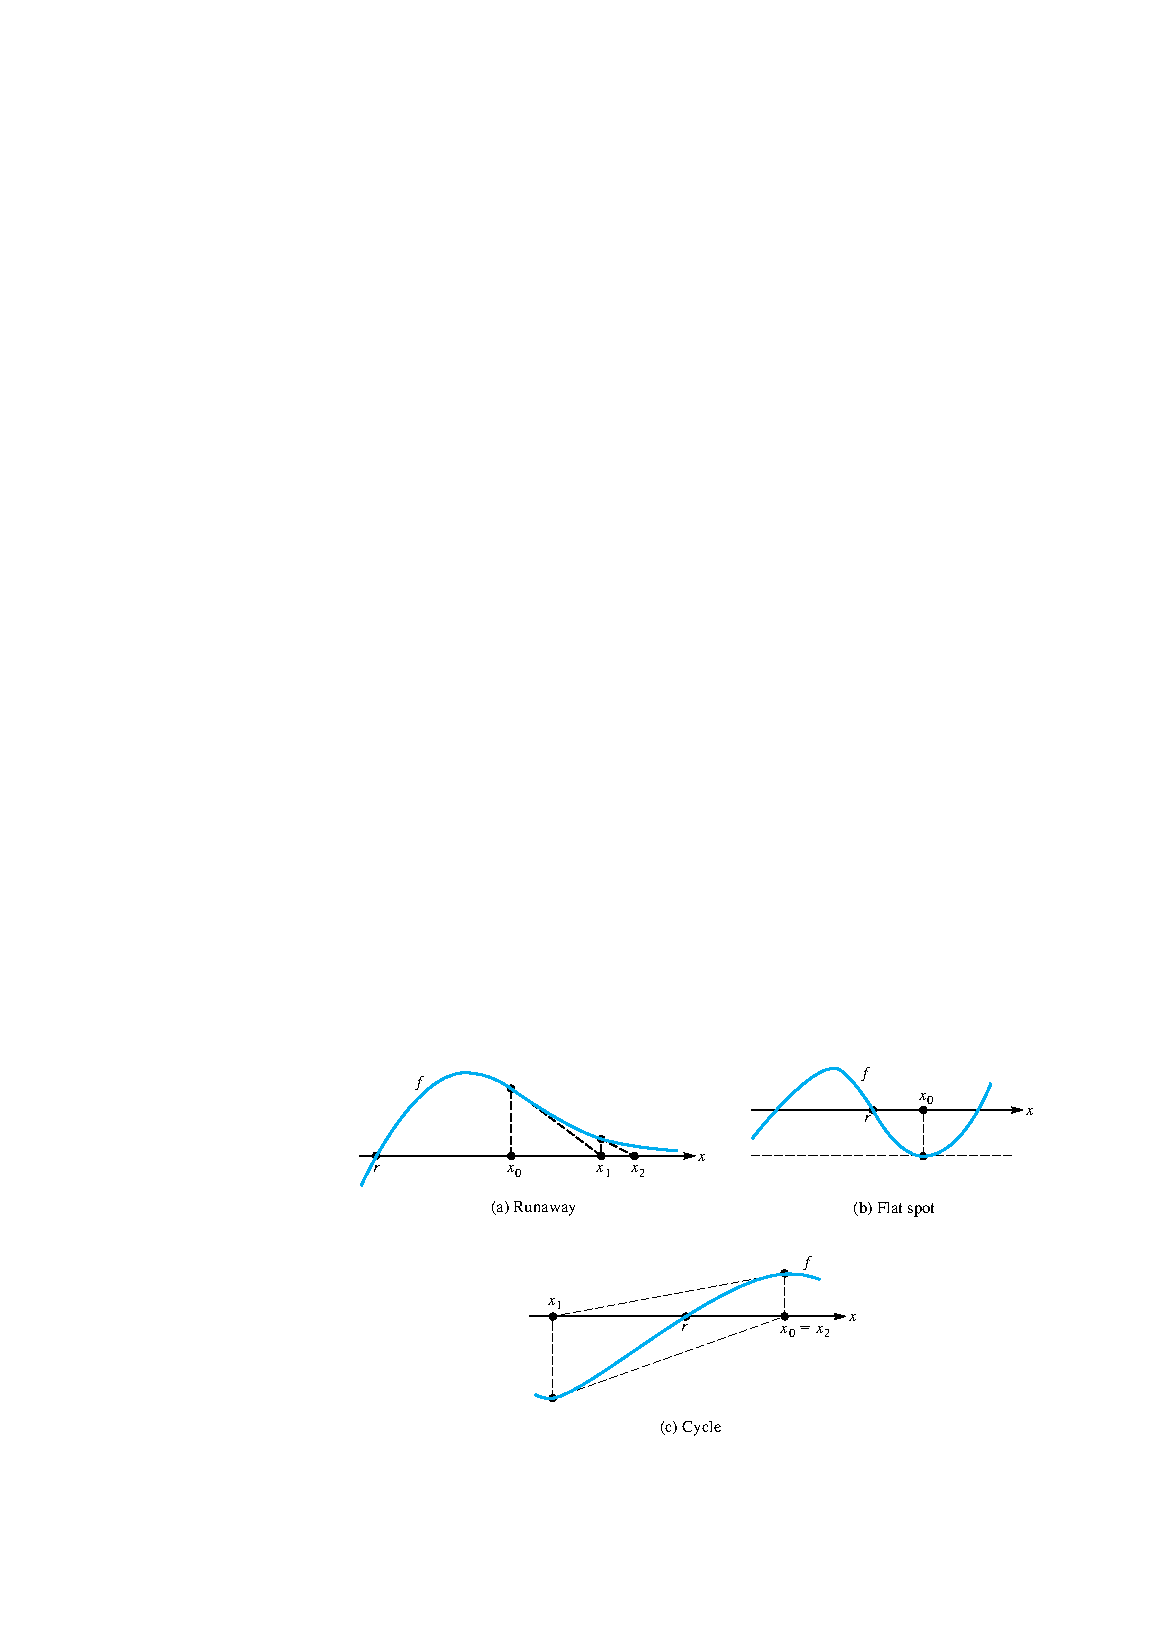
\includegraphics[height=1.5in]{Lec11_fig6.pdf}}
  \begin{itemize}
    \item In the use of Newton's method, consideration must be given to the proper choice of a starting point. 
    \item  Its convergence depends upon hypotheses that are difficult to verify a priori.
  \end{itemize}
\end{frame}

\subsection{Zeros of Polynomials}
\begin{frame}{Zeros of Polynomials}
\begin{itemize}
  \item A polynomial of degree $n$ has the form 
    $$
    P_n(x)=a_0+a_1 x+a_2 x^2+\cdots+a_n x^n,
    $$
     where the coefficients $a_i$ may be real or complex.
  \item $P_n(x)=0$ has $n$ roots, which may be real or complex.
  \item If the coefficients $a_i$ are real, then the roots of $P_n(x)$ are either real or occur in complex conjugate pairs.
\end{itemize}
\end{frame}

\begin{frame}[fragile]
  \frametitle{ Evaluation of Polynomials}
\begin{itemize}
  \item If we naively evaluate  $P_n(x)$ at a point $x$ by the simple algorithm
  \begin{verbatim}
    p=0.0
    for i in range(n+1):
        p+=a[i]*x**i
    \end{verbatim}
  \item The number of multiplications is $n(n+1)/2$ and the number of additions is $n$.
  \item The Horner's method is a more efficient way to evaluate a polynomial.
\end{itemize}
\end{frame}

\begin{frame}{Horner's Algorithm}
$$
\begin{aligned}
p(x) & =a_0+a_1 x+a_2 x^2+\cdots+a_{n-1} x^{n-1}+a_n x^n \\
& =a_0+x\left(a_1+x\left(a_2+\cdots+x\left(a_{n-1}+x\left(a_n\right)\right) \cdots\right)\right)
\end{aligned}
$$
\begin{itemize}
  \item Exponentiations are dangerous.
  \item The algorithm can be used to deflate a polynomial
\end{itemize}

\[
\begin{gathered}
p(x)=(x-r) q(x)+p(r) \\
q(x)=b_0+b_1 x+b_2 x^2+\cdots+b_{n-1} x^{n-1}
\end{gathered}
\]

\end{frame}
\begin{frame}{Polynomial Division}
$$
\begin{aligned}
p(x) & =a_0+a_1 x+a_2 x^2+\cdots+a_{n-1} x^{n-1}+a_n x^n \\
& =a_0+x\left(a_1+x\left(a_2+\cdots+x\left(a_{n-1}+x\left(a_n\right)\right) \cdots\right)\right)
\end{aligned}
$$
$$
\begin{aligned}
p\left(x_0\right) & =a_0+x_0\left(a_1+x_0\left(a_2+\cdots+x_0\left(a_{n-1}+b_n x_0\right) \cdots\right)\right) \\
& =a_0+x_0\left(a_1+x_0\left(a_2+\cdots+x_0\left(b_{n-1}\right) \cdots\right)\right) \\
& \vdots \\
& =a_0+x_0\left(b_1\right) \\
& =b_0
\end{aligned}
$$
$$
b_n  =a_n, \quad b_{n-1}=a_{n-1}+b_n x_0, \quad \ldots, \quad b_0=a_0+b_1 x_0
$$

$$
p(x)=\left(x-x_0\right)\left(b_n x^{n-1}+b_{n-1} x^{n-2}+\cdots+b_1\right)+b_0
$$
\end{frame}

\begin{frame}{Lagguerre's Method}
  \begin{itemize}
    \item Laguerre's method is a root-finding algorithm that is particularly effective for finding the roots of polynomials.
    \item Consider a special polynomial $P_n(x)=(x-r)(x-q)^{n-1}$, where $r$ and $q$ are the roots of $P_n(x)$.
    \item Given $P_n(x)=a_0+a_1 x+a_2 x^2+\cdots+a_n x^n$, find the root $r$ of $P_n(x)$ (assuming $q$ is unknown).
    \item We can show 
    $$
    \frac{P_n^{\prime}(x)}{P_n(x)}=\frac{1}{x-r}+\frac{n-1}{x-q}, \quad \frac{P_n^v(x)}{P_n(x)}-\left[\frac{P_n^v(x)}{P_n(x)}\right]^2=-\frac{1}{(x-r)^2}-\frac{n-1}{(x-q)^2}.
    $$
  \end{itemize}
\end{frame}

\begin{frame}{Lagguerre's Method}
  \begin{itemize}
    \item Define $G(x)=\frac{P_n^{\prime}(x)}{P_n(x)} \quad H(x)=G^2(x)-\frac{P_n^{\prime \prime}(x)}{P_n(x)}$. 
    $$
G(x)=\frac{1}{x-r}+\frac{n-1}{x-q}, \quad H(x) =\frac{1}{(x-r)^2}+\frac{n-1}{(x-q)^2}.
$$
\item Eliminatng $x-q$ from $G(x)$ and $H(x)$, we obtain
$$
x-r=\frac{n}{G(x) \pm \sqrt{(n-1)\left[n H(x)-G^2(x)\right]}}
$$
  \end{itemize}
\end{frame}
\begin{frame}{Lagguerre's Method}
  \begin{multicols}{2}
    
\tiny
  \begin{algorithmic}
  \State \textbf{Input:} $P(x)$: Polynomial of degree $n$
  \State \textbf{Input:} $x_0$: Initial guess for the root
  \State \textbf{Input:} $max\_iter$: Maximum number of iterations
  \State \textbf{Input:} $tol$: Tolerance for convergence
  \State \textbf{Output:} Approximate root of the polynomial $P(x)$
  
  \State Define $P'(x)$ as the first derivative of $P(x)$
  \State Define $P''(x)$ as the second derivative of $P(x)$
  \State Set $x = x_0$
      
  \For{$k = 1$ to $max\_iter$}
      \State Compute $G = \frac{P'(x)}{P(x)}$
      \State Compute $H = G^2 - \frac{P''(x)}{P(x)}$
      
      \State Set $n$ as the degree of the polynomial $P(x)$
      
      \State Compute $D_1 = G + \sqrt{(n-1)\left(nH - G^2\right)}$
      \State Compute $D_2 = G - \sqrt{(n-1)\left(nH - G^2\right)}$
      
      \If{$|D_1| > |D_2|$}
          \State Set $D = D_1$
      \Else
          \State Set $D = D_2$
      \EndIf
      
      \State Update $x_{\text{new}} = x - \frac{n}{D}$
      
      \If{$|x_{\text{new}} - x| < tol$}
          \State \Return $x_{\text{new}}$ (Root found)
      \EndIf
      
      \State Set $x = x_{\text{new}}$
  \EndFor
  
  \State \Return failure if no root found within $max\_iter$ iterations.
  
  \end{algorithmic}
\end{multicols}

\end{frame}
\end{document}


